\documentclass{article}

\usepackage{graphicx}
\graphicspath{ {./images/} }

\title{HW 10.3. Solutions}
\author{Principles of Microeconomics}
\date{\today}

\begin{document}

\maketitle

\subsection*{Quick Quiz}

\begin{enumerate}
\setcounter{enumi}{6}

\item (a) -- The Coase Theorem states that if private parties can bargain without cost, they can solve the problem of externalities without government intervention.

\item (c) -- Bargaining must be low cost for the Coase Theorem to apply.

\end{enumerate}

\subsection*{Problems \& Applications}

\begin{enumerate}
\setcounter{enumi}{5}

\item

	\begin{enumerate}
	
	\item Bruno's loud rock creates a negative externality because Placido can probably hear it through the wall, and she dislikes rock.
	
	\item The land lord could ban loud music. That policy could lead to an inefficient outcome though because the loud music might create a bigger benefit for Bruno than it creates a cost for Placido.
	
	\item Placido could offer to pay Bruno to turn down his music. If Placido's costs from hearing the rock are greater than Bruno's benefits, she would eventually offer him a price that exceeds his benefits, and he would turn down his music. When her costs exceed his benefits, that's the efficient outcome. If Placido's costs are less than Bruno's benefits she would never offer him a price that exceeds his benefits, and he would continue playing his music at high volume. When his benefits exceed her costs, that's the efficient outcome.
	
	If there are transaction costs to their negotiation, they might not reach the efficient outcome. For example, they might not speak the same language, or they may detest each other from some prior dispute. In both cases, negotiating becomes onerous, so they might not reach an agreement.
	
	\end{enumerate}
	
\newpage
	
\item

	\begin{enumerate}
	
	\item \phantom{x}
	
		\begin{center}
		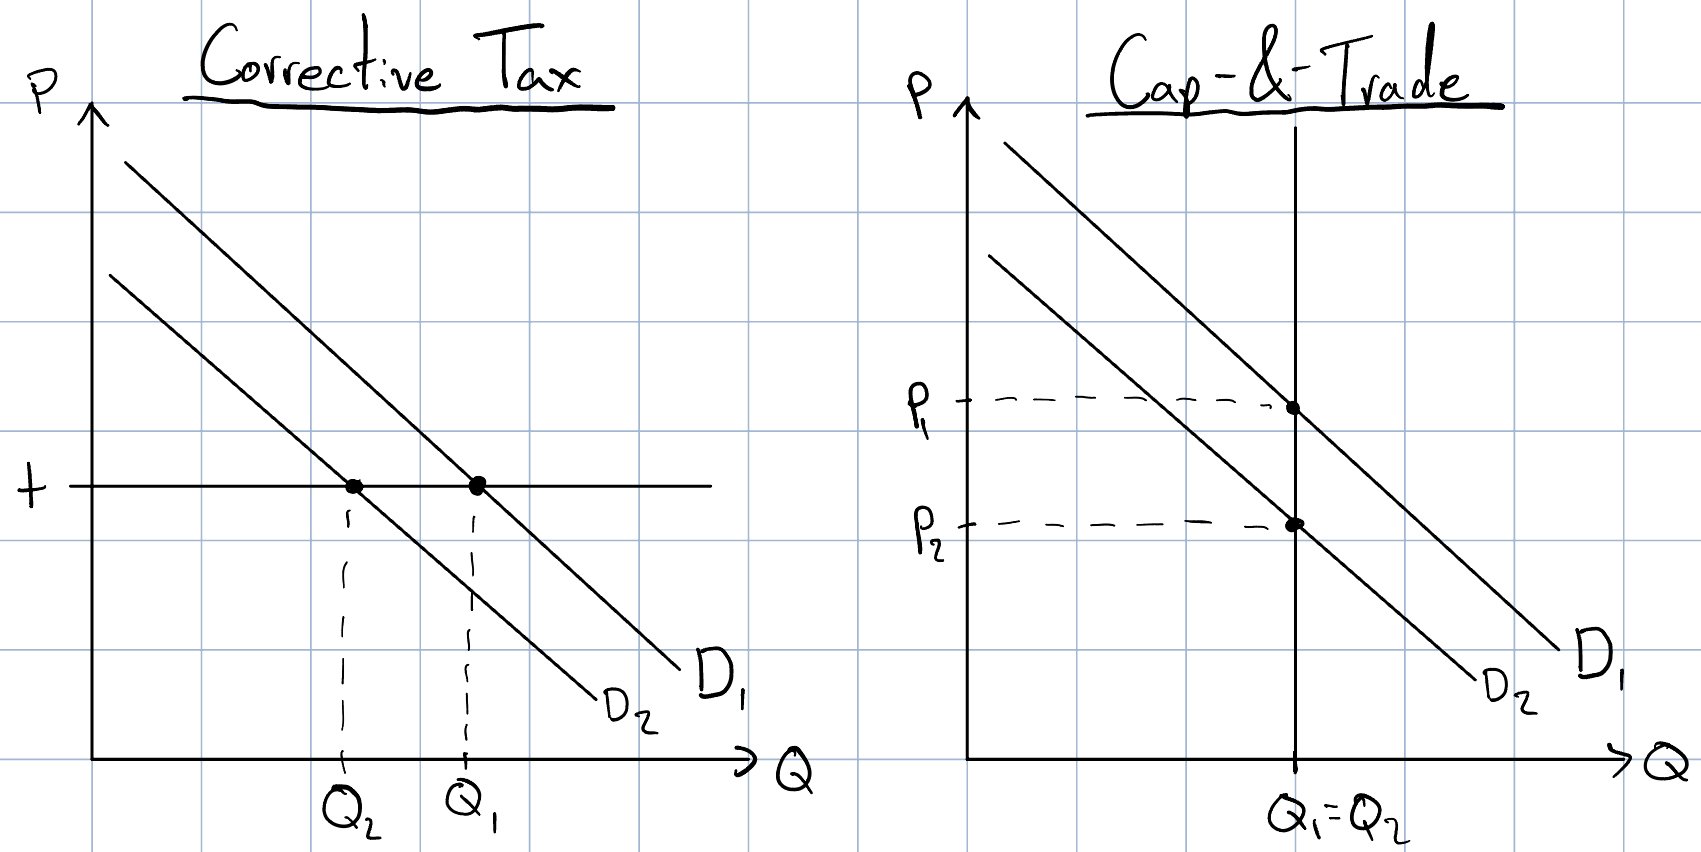
\includegraphics[width = \textwidth]{paa7a}
		\end{center}
		
	\item The improvement in technology for controlling pollution will decrease the demand for pollution. Under the corrective tax, the price of polluting remains constant at the level of the tax, but the quantity of pollution goes down. Under the cap-and-trade policy, the quantity of pollution will remain fixed at the capped amount, but the price of polluting will go down because the permits will be less valuable.
	
	\end{enumerate}
	
\item

	\begin{enumerate}
	
	\item It does not. Under an auction system, the firms that value polluting the most will win the permits. Under a distribution system, the permits are tradable, so the firms that value polluting more will buy the permits from firms who value polluting less. The firms who value polluting more will be the firms who face higher costs for reducing their pollution. Therefore, under both systems, we get the efficient outcome because the firms who face higher costs will reduce their pollution less and the firms who face lower costs will reduce their pollution more.
	
	\item It does not. The firms who value them more will buy them from the firms who value them less. As a result, the firms who face high costs for reducing their pollution will reduce less, and the firms who face low costs will reduce more. 
	
	\end{enumerate}

\end{enumerate}

\end{document}